\documentclass{article}
\usepackage{amsmath,amssymb}
\usepackage[T1]{fontenc}
\usepackage[utf8]{inputenc}
\usepackage{textcomp}
\newcommand{\midtilde}{\raisebox{-0.25\baselineskip}{\textasciitilde}}
\usepackage{graphicx}
\usepackage{float}
\graphicspath{ {./images/} }

\begin{document}

\section*{Bayesian network: example}
\begin{figure}[H]
 \centering 
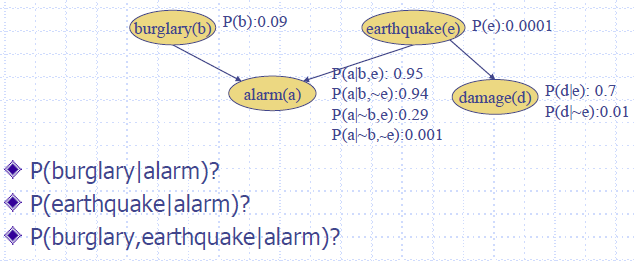
\includegraphics[scale=0.65]{images/alarm.png} 
 \caption{Bayesian network: example}
 \label{fig:b-net-example}
\end{figure}

\begin{align*}
p(b|a) ? & \\
p(e|a) ? & \\
p(b,e|a) ? & \\
p(a) & = p(a,b) + p(a,e) \\
p(a,b) & = p(a,b,e) + p(a,b,\midtilde e) \\
p(a,b,e) & = p(e)p(b)p(a|b,e) \\
p(a,b,\midtilde e) & = p(\midtilde e)p(b)p(a|b,\midtilde e) \\
p(a,e) & = p(a,b,e) + p(a,\midtilde b,e) \\
p(a,\midtilde b,e) & = p(e)p(\midtilde b)p(a|\midtilde b,e) \\
p(b|a) & = \frac{p(a,b)}{p(a)} \\
p(e|a) & = \frac{p(a,e)}{p(a)} \\
p(b,e|a) & = \frac{p(e)p(b)p(a|b,e)}{p(a)} \\
\end{align*}

\end{document}